\documentclass{tufte-handout}

\title{Utility Theory and the Representation of Preference}

\author[Nathaniel Forde]{Nathaniel Forde}

%\date{28 March 2010} % without \date command, current date is supplied

%\geometry{showframe} % display margins for debugging page layout

\usepackage{graphicx} % allow embedded images
  \setkeys{Gin}{width=\linewidth,totalheight=\textheight,keepaspectratio}
  \graphicspath{{graphics/}} % set of paths to search for images
\usepackage{amsmath}  % extended mathematics
\usepackage{booktabs} % book-quality tables
\usepackage{units}    % non-stacked fractions and better unit spacing
\usepackage{multicol} % multiple column layout facilities
\usepackage{lipsum}   % filler text
\usepackage{fancyvrb} % extended verbatim environments
  \fvset{fontsize=\normalsize}% default font size for fancy-verbatim environments
\usepackage{minted}
\usepackage{mathtools}
\usepackage[math]{cellspace}

% Standardize command font styles and environments
\newcommand{\doccmd}[1]{\texttt{\textbackslash#1}}% command name -- adds backslash automatically
\newcommand{\docopt}[1]{\ensuremath{\langle}\textrm{\textit{#1}}\ensuremath{\rangle}}% optional command argument
\newcommand{\docarg}[1]{\textrm{\textit{#1}}}% (required) command argument
\newcommand{\docenv}[1]{\textsf{#1}}% environment name
\newcommand{\docpkg}[1]{\texttt{#1}}% package name
\newcommand{\doccls}[1]{\texttt{#1}}% document class name
\newcommand{\docclsopt}[1]{\texttt{#1}}% document class option name
\newenvironment{docspec}{\begin{quote}\noindent}{\end{quote}}% command specification environment

\begin{document}

\maketitle% this prints the handout title, author, and date

\begin{abstract}
\noindent
This article continues the investigation of the expected utility model of rational choice. We begin by examining the useful properties of utility functions, before continuing to the representation theorems which formalise the connection. Will we see that the nature of these theorems, coupled with the indeterminacy of statistical inference is a brittle foundation for predictive economic models of consumer choice.
\end{abstract}


\section{From Utility to Indifference}
Too much of a good thing often tends to the bad. So we dabble, sample and share. In pursuit of variety we swap our goods, shunning stale options in favour of the novel exchange.  For a given good we can differ in our appetites but it's relatively straightforward to find the point where one more donut is one too many. While it can be a bit unclear how we should measure utility, once we've decided on a metric the mathematical characteristics are meaningful. We can infer aspects of your attitudes towards acquisition and enthusiasm for donuts. In most cases we're interested not just in your pursuit of pastries, but how you'd be willing to trade for those pastries. 

\begin{marginfigure}
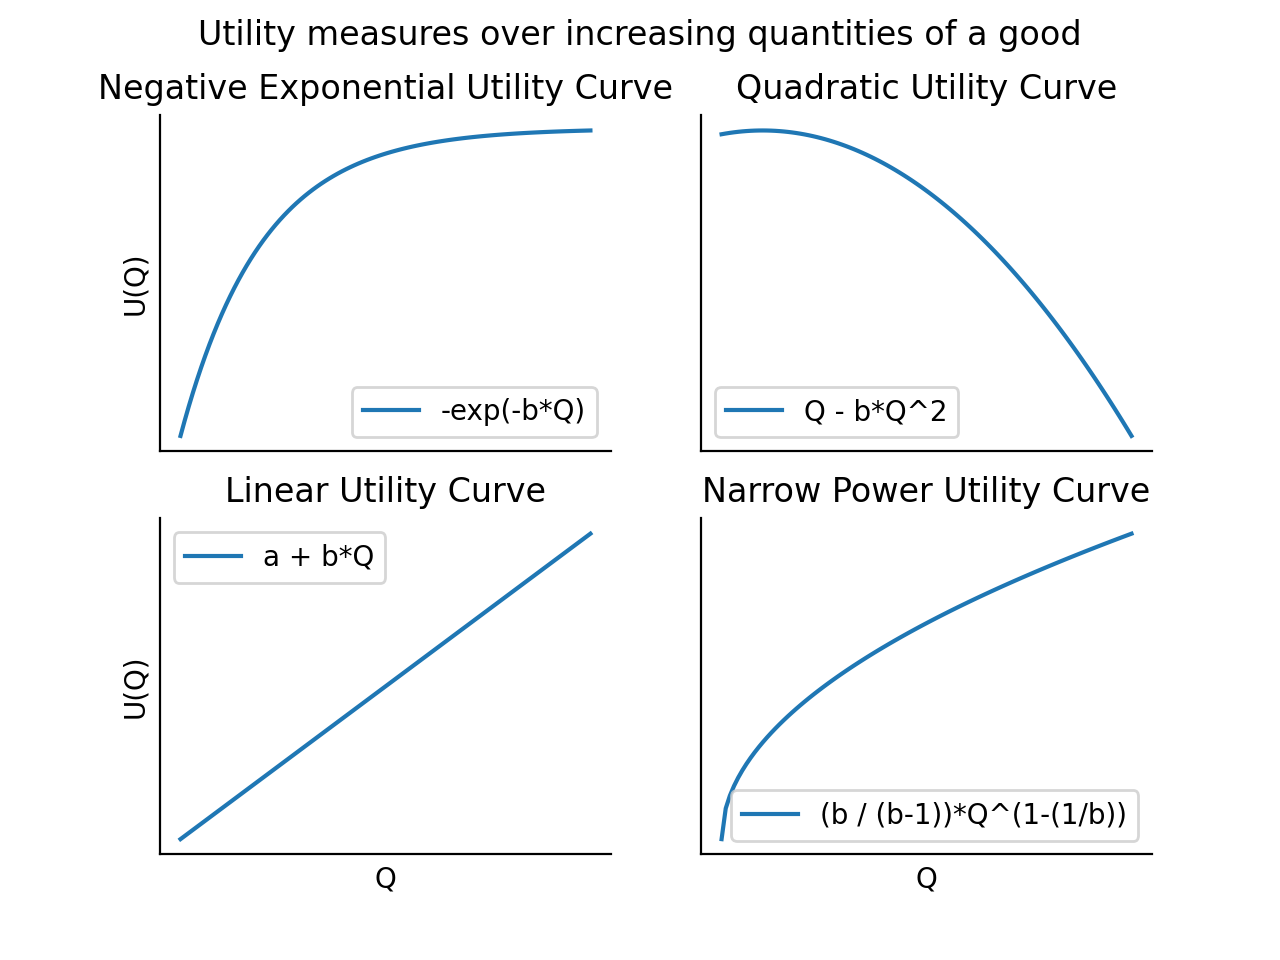
\includegraphics[width=3in]{Plots/utility_in_1_dimension.png}
\caption{Consumer attitudes with differently satisfied appetites for a good}
\includegraphics[width=3in]{Plots/derivatives_of_utility.png}
\caption{The Rates of Change of personal Utility}
\end{marginfigure} 

The possibility of coordinated compromise lies at the core of maximising subjective utility. We seek competitive advantage for our own produce to balance the cost owed to the skills of others. At the limit some trades do not admit any mixture of goods. Not all babies can be cut in half. On the other side of the spectrum, there are some things which we'd give everything. In most cases though a consumer will try to optimise their bundle of goods over an entire marketplace, preserving enough on one key good; money, to remain liquid. 

$$ u(\mathbf{g}) = f(g_{0}, g_{1} ... g_{n}) $$

There are number of ways we can specify a utility function, but a typical example is the Cobb-Douglas function. 

$$ u(\mathbf{g}) = g_{0}^{\alpha_{0}}g_{1}^{\alpha_{1}} ... g_{n}^{\alpha_{n}}$$

\begin{marginfigure}
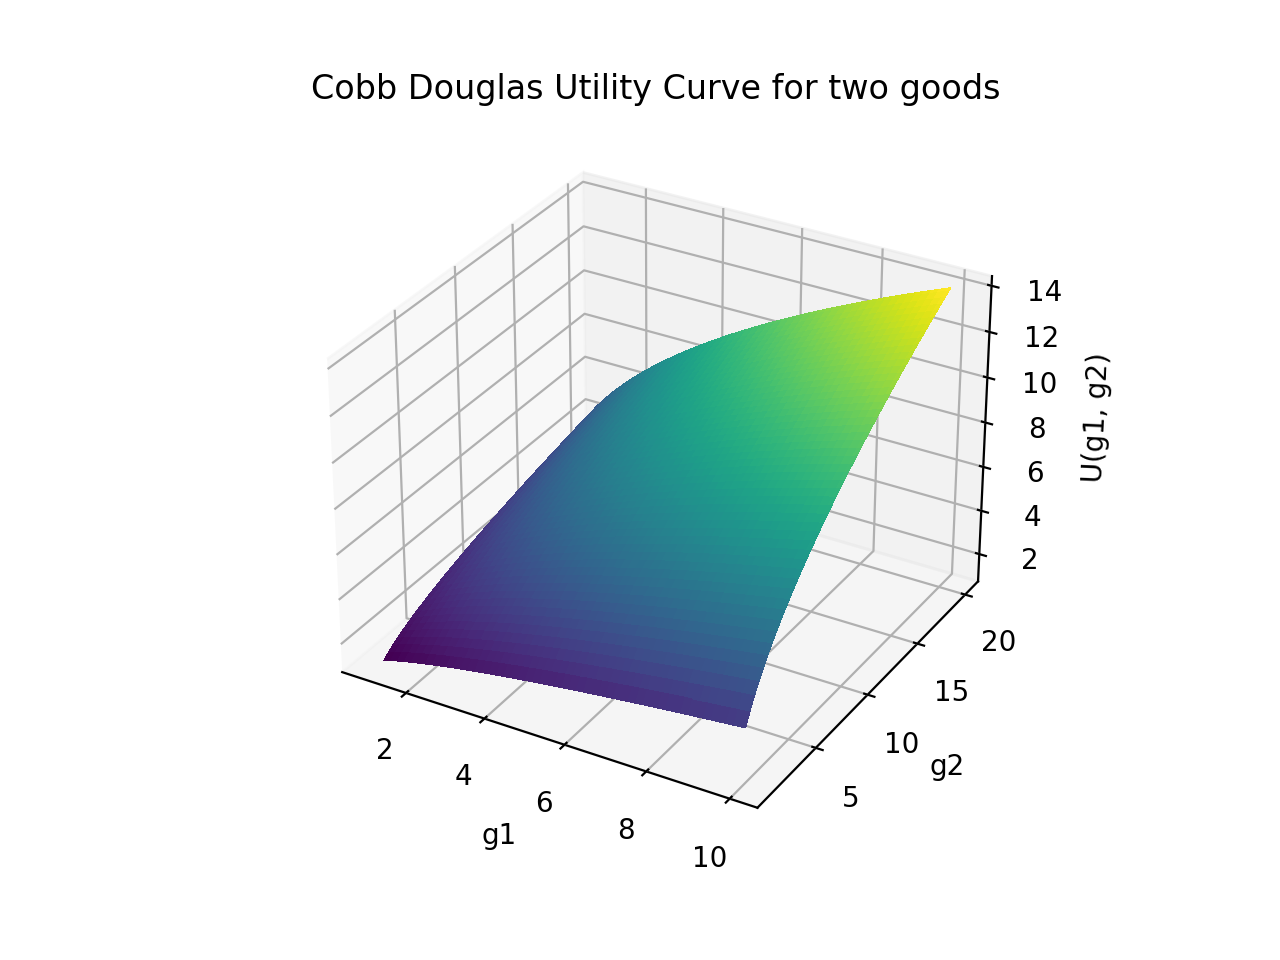
\includegraphics[width=3.2in, height=5.in]{Plots/cobb_douglas_utility.png}
\caption{A consumers utility curve for combinations of two goods}
\end{marginfigure} 

Then taking the case of two goods $g1, g2$ we can in this particular case determine an indifference curve where you would be willing to exchange quantities of $g1$ for an agreeable amount of $g2$.  Set 
$$u(\mathbf{g}) = k =  g_{1}^{\frac{1}{2}}g_{2}^{\frac{1}{2}} = (g_{1}g_{2})^{\frac{1}{2}}  = \sqrt{g_{1}g_{2}}$$
$$ \Rightarrow k^{2} = g_{1}g_{2} \Rightarrow \frac{k^{2}}{g_{2}} = g_{1}$$

Using this formula we can express how the quantities of fair exchange vary based on a fixed utility value. This is not to say that these curves represent an actual or objective fair price, just that when measured in terms of utility these are mappings of quantities of good we would be happy to exchange. Your view of a fair price is encoded in your utility theory. It's at this point when utility theory can be said to verge on empirical science.If we can model your preferences as a utility function characteristic of some general attitude toward acquisition, we might also hope to able to predict future trades.  
\begin{marginfigure}
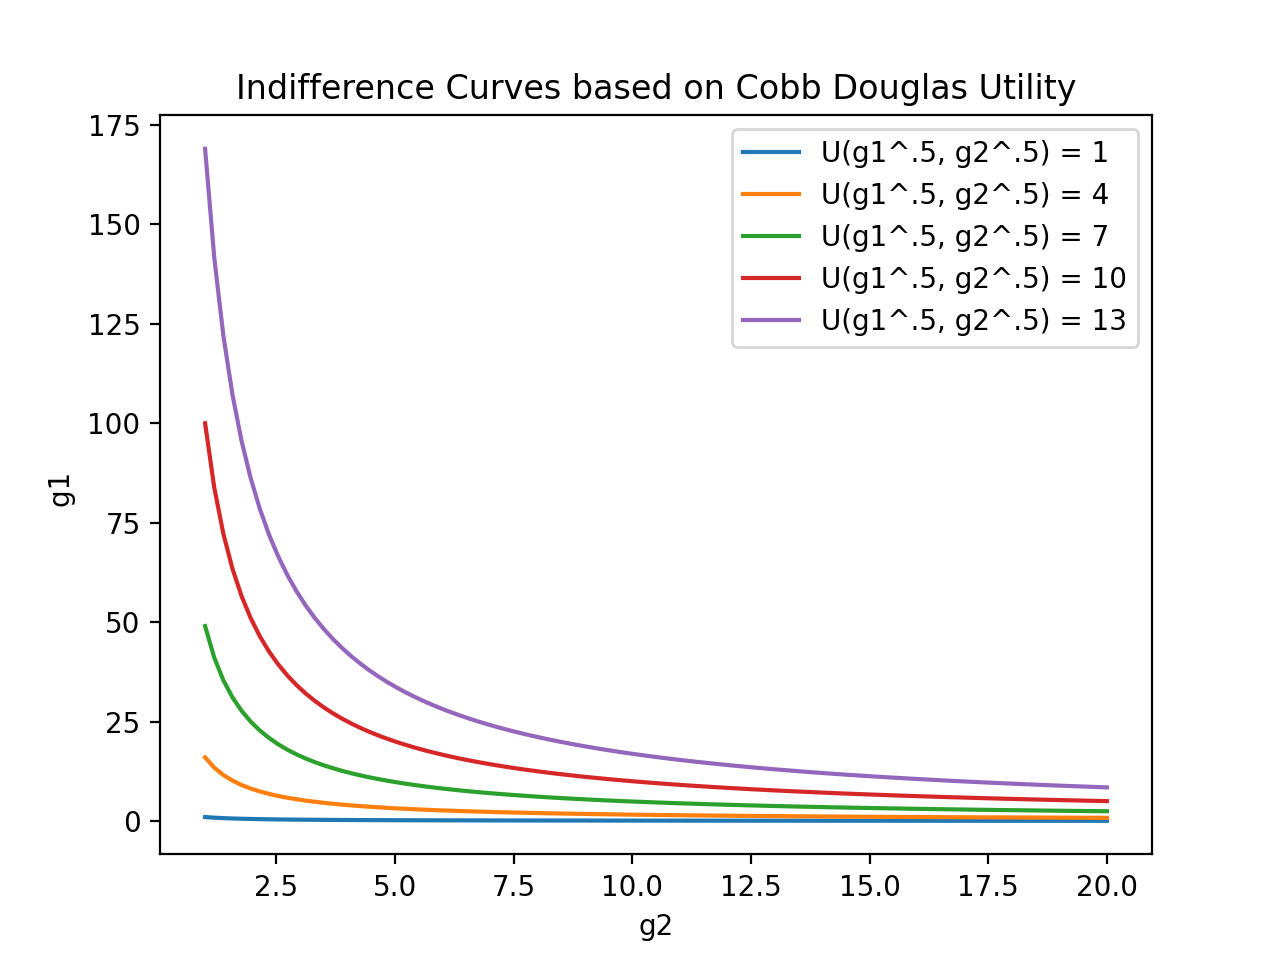
\includegraphics[width=3in, height=5.in]{Plots/indifference_curves.png}
\caption{A range of indifference curves without budget constraints.}
\end{marginfigure}

\subsection*{Optimising Utility}
A further complication arises when  we try to factor for a consumer's budget. The shape of the Cobb-Douglas function shows that the utility surface is constantly increasing with our rate acquisition. So without any constraints the consumer would not achieve satisfaction, but continue like glutton. But add a budget constraint and we need to find the maximum point at which an indifference curve insects with our budgetary line. Instead of solving the equation: 

$$ \text{ Find } g_{1}, g_{2} \text{ such that } u(g_{1}, g_{2}) = k $$

\noindent we need to solve a constrained optimisation problem: 
$$ \text{ maximise } u(g_{1}, g_{2})  \text{ subject to } cost(g_{1}, g_{2}) =  k$$

\noindent This style of problem can be approached with the method of Lagrange multipliers. If we let:

\begin{marginfigure}
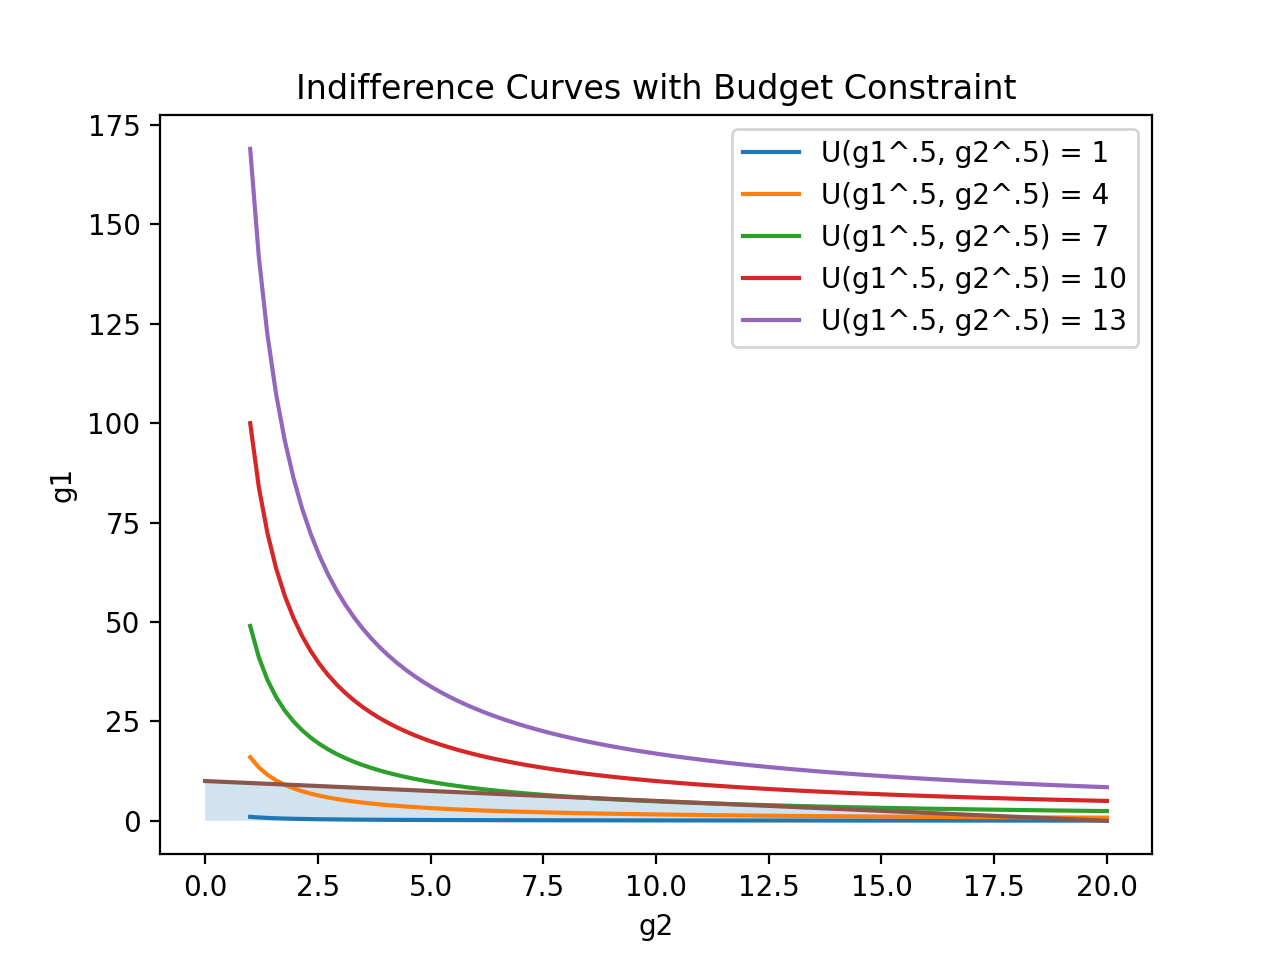
\includegraphics[width=3in, height=5.in]{Plots/indifference_curves_budget.png}
\caption{A range of indifference curves with budget constraints.}
\end{marginfigure}

$$ L = g_{1}^{\frac{1}{2}}g_{2}^{\frac{1}{2}} - \lambda(2g_{1} + 3g_{2} - 40) $$

\noindent where $2$ and $3$ are the unit cost of the respective goods, and $40$ is our total budget. While $\lambda$ is our Lagrangian multiplier. This term will be used to re-express the algebra of our equation as a function of the consumer's capacity to spend. We can discover where utility is maximised when its gradient can be set to zero. As before we first want to express the implicit function of $g_{1}$ in terms of $g_{2}$, but this time including the constraints.


\[
\nabla L = dL /  d\mathbf{g} =
    \begin{pmatrix}
       \dfrac{\partial u(\mathbf{g})}{\partial g_1}   & , \dfrac{\partial u(\mathbf{g})}{\partial g_2}
    \end{pmatrix} = \begin{pmatrix}
    \frac{1}{2}g_{1}^{-\frac{1}{2}}g_{2}^{\frac{1}{2} } - 2\lambda & ,
    \frac{1}{2}g_{2}^{-\frac{1}{2}}g_{1}^{\frac{1}{2} } - 3\lambda
    \end{pmatrix} = \mathbf{0}
  \]


$$ \Rightarrow \lambda = \frac{1}{4}g_{1}^{-\frac{1}{2}}\sqrt{g_{2}} = \frac{4}{25}g_{2}^{-\frac{1}{2}}\sqrt{g_{1}}$$

$$ \Rightarrow  (\frac{1}{4})^2\frac{1}{g_{1}}g_{2} = (\frac{4}{25})^2\frac{1}{g_{2}}g_{1} \Rightarrow (\frac{1}{4})^2 g_{2} = (\frac{4}{25})^2\frac{1}{g_{2}}g_{1}^2  \Rightarrow (\frac{1}{4})^2g_{2}^{2} = (\frac{4}{25})^2g_{1}^2 $$ 

$$ \Rightarrow g_{2} = \frac{16}{25}g_{1}$$

\noindent The same pattern holds for cases with more than two goods. We can express the value of given good $g_n$ in terms of a function $f(g_{1}, ... g_{n-1}) $. Then substituting this value into our constraint we get: 

$$ 2g_{1} + 3(\frac{16}{25})g_{1} = 40 \Rightarrow 2g_{1} + 1.92g_{1} = 40 \Rightarrow 3.92g_{1} = 40$$
$$ \text{ Proving the optimial settings are } g_{1}^{*} = 10.20 \text{ and } g_{2}^{*} = 6.52 \text{ and } \lambda^{*} = 0.20 $$

Furthermore, we can interpret the $\lambda$ term as the rate of change of the consumer's utility as a function of the cost. The proof is a little more involved, but the significance of this interpretation should be obvious. If we knew our consumer's adhered to a particular style of utility function we could model how price-changes would impact their returns to utility. 

\subsection*{Estimating Utility Curves from Expressed Preference}

If we can elicit preference statements from our consumer we construct a utility curve as follows. First observe the preferences expressed by consumer decisions and then map the maximal and least preferred options to convenient polarities. For instance:

$$ g_{1} \succ g_{2} \succ g_{3} \succ g_{4} \succ g_{5} $$

where:

$$ u(g_{1}) = 0 \text{ and } u(g_{5}) = 1 $$

\noindent then each of the intermediary options can be measured in the interval between 0 and 1. However there are an infinite number of simple ordinal mappings that would work, and a strict ordering does nothing to convey the degree of feeling associated with each option. 




\bibliography{sample-handout}
\bibliographystyle{plainnat}



\end{document}
